\section{Auswertung}
\label{sec:auswertung}
	% Im Folgenden werden alle Schwingungsdauertn $T$ "uber drei Perioden gemessen und gemittelt.
	% Zudem werden jeweils 10 Messungen vorgenommen und ein Mittelwert $\overline{T}$ mit der Standardabweichung $\sigma$ gebildet.

	Im Folgenden wird "uber alle Messungen ein Mittelwert $\overline{T}$ mit Standardabweichung $\sigma$ gebildet.
	Bei einer Anzahl von $n$ Stichproben gilt

	\begin{eqnarray}
		\overline{T} & = & \frac{1}{n} \sum_{i = 1}^n{T_i} \nonumber \\
		%\sigma_T = \sqrt{\frac{1}{n-1}\sum_{i = 1}^n {(T_i - \overline{T})^2}} \,.
		\Delta T & = & \left(\frac{1}{n-1}\sum_{i = 1}^n {(T_i - \overline{T})^2}\right)^{\frac{1}{2}} \,. \nonumber
	\end{eqnarray}

	%Der Ablesefehler bei L"angenbestimmung liegt bei allen Werten bei $\Delta x = \SI{.5}{\milli \meter}$.

	\subsection{Bestimmung der Winkelrichtgr"o"se $D$}
	\label{subsec:winkelrichtgroesse}
		%Zun"achst muss die Winkelrichtgr"o"se $D$ aus Gleichung \eqref{eqn:richtgroesse} bestimmt werden.
		Die Winkelrichtgr"o"se berechnet sich nach

		\begin{equation*}
			D = \frac{F \cdot r}{\varphi} \,.
		\end{equation*}

		Tabelle \ref{tabelle:winkelrichtgroesse} zeigt die Messwerte.
		Die Winkel wurden in Radianten umgerechnet.
		F"ur die Winkelrichtgr"o"se erh"alt man damit

		\begin{equation*}
			D = \SI{19.9 (43)}{\milli \newton \meter \per \radian} \,.
		\end{equation*}

		Berechnet man mit diesem Wert jedoch das Eigentr"agheismoment der Apparatur, ergeben sich negative Werte.
		Ein besserer Wert ergibt sich durch eine lineare Ausgleichsrechnung, die im folgenden Kapitel \ref{subsec:eigentraegheitsmoment} durchgef"uhrt wird.
		% Diese ergibt

		% \begin{equation*}
		% 	D = \SI{57.9 (3)}{\milli \newton \meter} \,.
		% \end{equation*}

		\begin{table}[h!]
			\begin{center}
				\caption{Messwerte f"ur die Bestimmung der Winkelrichtgr"o"se $D$ \label{tabelle:winkelrichtgroesse}}
				\begin{tabular}{|c|c|c|c||c|c|c|c|}
					\hline
					$r [\SI{}{\centi \meter}]$ & $\varphi [\SI{}{\degree}]$ &  $F [\SI{}{\milli \newton}]$ & $D \left[\SI{}{\milli \newton \meter \per \radian}\right]$ & $r [\SI{}{\centi \meter}]$ & $\varphi [\SI{}{\degree}]$ &  $F [\SI{}{\milli \newton}]$ & $D \left[\SI{}{\milli \newton \meter \per \radian}\right]$\\
					\hline 
					\hline
					20	&	 10	&	10 & 2,00 & 20	&	 60	&	33 & 3,63 \\
20	&	 20	&	16 & 2,50 & 20	&	 71	&	35 & 4,05 \\
20	&	 30	&	20 & 3,00 & 20	&	 80	&	38 & 4,21 \\
20	&	 41	&	23 & 3,56 & 20	&	 90	&	44 & 4,09 \\
20	&	 50	&	27 & 3,70 & 20	&	101	&	50 & 4,04 \\





					\hline 
				\end{tabular}
			\end{center}
		\end{table}

	\subsection{Bestimmung des Eigentr"agheitsmomentes $I_\mathrm{D}$ der Drehachse}
	\label{subsec:eigentraegheitsmoment}
		% Um den Einfluss des Eigentr"agheitsmomentes $I_\mathrm{D}$ der Apparatur auf die Messwerte zu bestimmen, muss dieses gemessen werden.
		Zur Messung des Eigentr"agheitsmomentes $I_\mathrm{D}$ der Drehachse werden zwei Gewichte der Masse $m$ im gleichen Abstand $a$ zur Drehachse an einem Metallstab der Masse $M$ und der L"ange $l$ angebracht.
		Das Gesamttr"agheitsmoment des Systems wird dann durch

		\begin{equation}
			I = I_\mathrm{D} + I_\mathrm{Stange} + 2 I_\mathrm{m} \, \label{eqn:gesamtmoment}
		\end{equation}

		beschrieben, wobei das Tr"agheitsmoment der Stange durch $I_\mathrm{stange}$ gegeben ist und $I_\mathrm{m}$ das Tr"agheitsmoment eines Gewichtes unter Ber"ucksichtigung des Steinerschen Satzes bezeichnen. 
		Die Stange wird dabei als langer Stab betrachtet.
		Es gilt mit der Masse $M$ und L"ange $l$ der Stange, sowie dem Abstand $a$ zwischen Drehachse und Mittelpunkt der Zusatzgewichte und deren Radius $r$ und H"ohe $h$:
		%Hierbei kann n"aherungsweise angenommen werden, dass f"ur gegen $a$ kleine Radien $r$ und geringe H"ohen $h$, der zylindrischen Gewichten, gilt:

		\begin{eqnarray*}
		%	I_\mathrm{m} = \frac{1}{4}mr^2 + \frac{1}{12}mh^2 + ma^2 \approx ma^2 \,.
			I_\mathrm{Stange} & = & \frac{1}{12} M l \,, \\
			I_\mathrm{m} & = & \frac{1}{4}mr^2 + \frac{1}{12}mh^2 + ma^2 \,.
		\end{eqnarray*}

		Das Tr"agheitsmoment der Zusatzgewichte besteht dabei aus einem, "uber die Messung konstanten Anteil $I_\mathrm{m,c}$ und dem Anteil durch den Steinerschen Satz $ma^2$.
		Mit den Messwerten
		
		\begin{figure}[h!]
			\begin{minipage}[t]{7cm}
				\begin{eqnarray*}
					M & = & \SI{96.28}{\gram} \, \\
					l & = & \SI{60}{\centi \meter} \,
				\end{eqnarray*}
			\end{minipage}
			\hfill
			\begin{minipage}[t]{7cm}
				\begin{eqnarray*}
					m & = & \SI{222.70}{\gram} \, \\
					h & = & \SI{3.00}{\centi \meter} \, \\
					r & = & \SI{2.75}{\centi \meter} \,
				\end{eqnarray*}
			\end{minipage}
		\end{figure}

		ergeben sich die Werte von $I_\mathrm{Stange}$ und $I_\mathrm{m,c}$ zu

		\begin{equation*}
			I_\mathrm{Stange} = \SI{2.89}{\gram \meter \squared} \qquad , \qquad I_\mathrm{m,c} = \SI{.058}{\gram \meter \squared} \,.
		\end{equation*}

		Die Gleichungen \eqref{dauer} und \eqref{eqn:gesamtmoment} liefern dann den Zusammenhang

		\begin{equation*}
			T^2 = \frac{4 \pi^2}{D} \left(I_\mathrm{D} + I_\mathrm{Stange} + 2\left(I_\mathrm{m,c} + ma^2 \right)\right) \,.
		\end{equation*}
		mit
		\begin{eqnarray*}
			B & = & I_\mathrm{D} + I_\mathrm{Stange} \Leftrightarrow I_\mathrm{D} = B - I_\mathrm{Stange} \\
			\Rightarrow \quad T^2 & = & \frac{4\pi^2}{D}\left(B + 2\left(T_\mathrm{m,c} + ma^2\right)\right) \,.
		\end{eqnarray*}

		Das Eigentr"agheitsmoment $I_\mathrm{D}$ kann also durch Messung von $T$ und $a$ mit einer Ausgleichsrechnung f"ur den Parameter $B$ bestimmt werden.
		Zudem l"asst sich mit dieser Rechnung $D$ bestimmen.
		Wie in Kapitel \ref{subsec:winkelrichtgroesse} erw"ahnt liefert diese Rechnung einen besseren Wert f"ur $D$.

		Die Ausgleichsrechnung durch \emph{python} liefert

		\begin{eqnarray*}
			B & = & \SI{5.33 (22)}{\gram \meter \squared} \\
			\Rightarrow \quad I_\mathrm{D} & = & \SI{2.44 (22)}{\gram \meter \squared} \,,
		\end{eqnarray*}

		sowie

		\begin{equation*}
			D = \SI{57.9 (3)}{\milli \newton \meter \per \radian} \,.
		\end{equation*}

		Die zur Berechnung genutzten Daten werden in Tabelle \ref{tabelle:eigentraegheitsmoment} aufgef"uhrt.
		Da das Eigentr"agheitsmoment jedoch gr"o"ser ist als die Tr"agheitsmomente der untersuchten Objekte, w"urden sich negative Tr"agheitsmomente ergeben.
		Das ergibt physikalisch keinen Sinn, weshalb $I_\mathrm{D}$ in den sp"ateren Rechnungen nicht abgezogen wird.

		\begin{table}[h!]
			\begin{center}
				\caption{Messwerte f"ur die Bestimmung des Eigentr"agheitsmomentes $I_\mathrm{D}$ \label{tabelle:eigentraegheitsmoment}}
				\begin{tabular}{|c|c||c|c|}
					\hline
					$a [\SI{}{\centi \meter}]$ & $\overline{T} [\SI{}{\second}]$ & $a [\SI{}{\centi \meter}]$ & $\overline{T} [\SI{}{\second}]$\\
					\hline 
					\hline
					26	&	20,16	& 16	&	13,12\\
26	&	20,13	& 16	&	13,16\\
24	&	18,60	& 14	&	11,75\\
24	&	18,50	& 14	&	11,72\\
22	&	17,18	& 12	&	10,53\\
22	&	17,22	& 12	&	10,53\\
20	&	15,78	& 10	&	09,34\\
20	&	15,88	& 10	&	09,37\\
18	&	14,69	& 08	&	08,31\\
18	&	14,64	& 08	&	08,25\\
					\hline 
				\end{tabular}
			\end{center}
		\end{table}

		\clearpage

		\begin{figure}[h!]
			\centering
			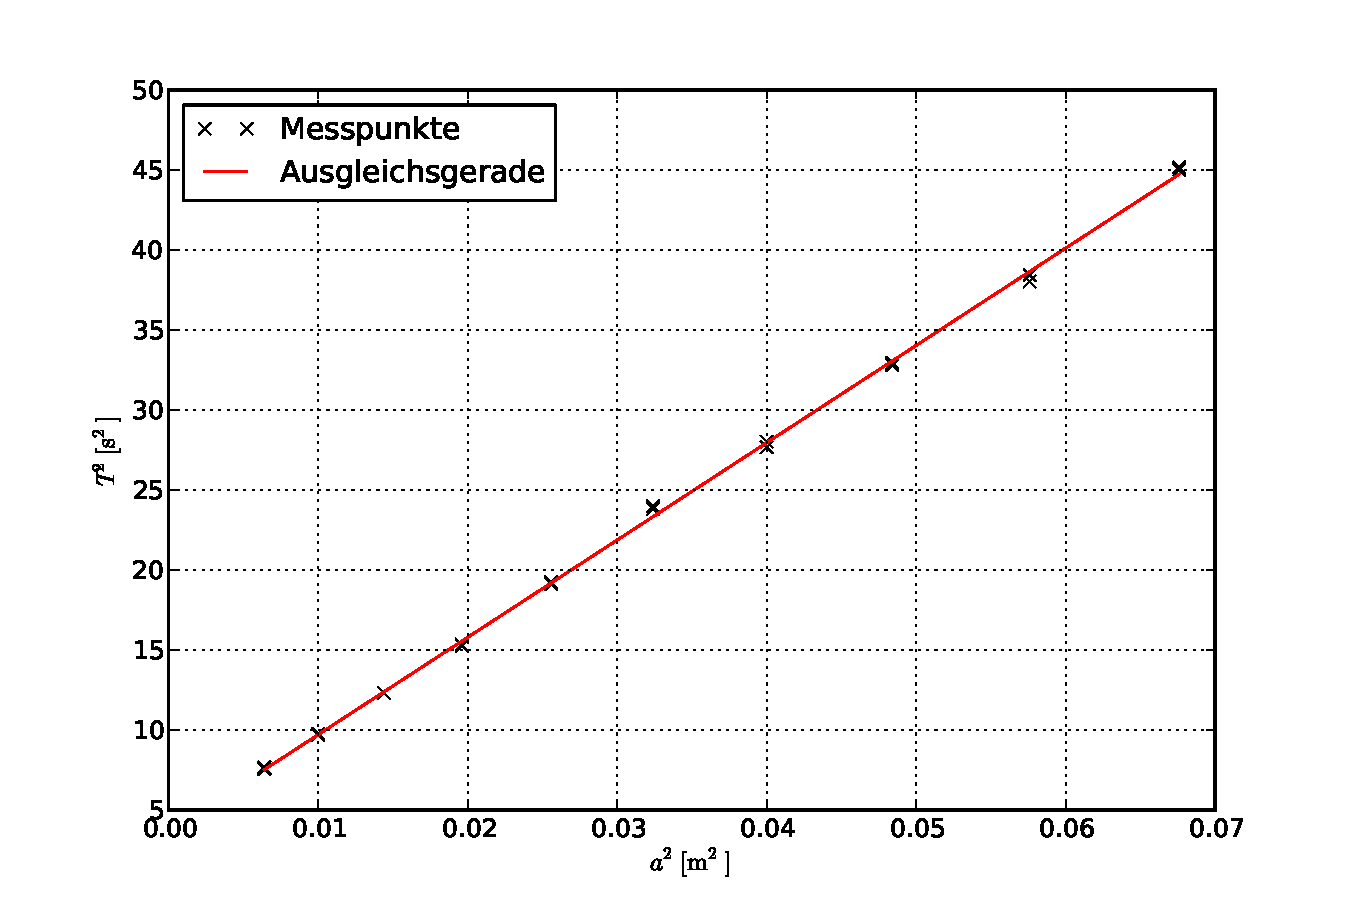
\includegraphics[width = 15cm]{img/graph2_T.pdf}
			\caption{Ausgleichsgerade zur Bestimmung von $I_\mathrm{D}$ und $D$}
			\label{fig:graph2}
		\end{figure}

		\subsection{Bestimmung der Tr"agheitsmomente $I_\mathrm{k}$ verschiedener K"orper}
		\label{subsec:versch_momente}
			% Schlie"slich werden die Tr"agheitsmomente $I_\mathrm{k}$ f"ur $k$ verschiedene K"orper bestimmt.
			% Dabei handelt es sich um eine Holzkugel, einen Messingzylinder, sowie eine Holzpuppe, die in zwei verschiedenen K"orperhaltungen eingespannt wird.

			Aus der Periodendauer wird gem"a"s Gleichung \eqref{dauer} das Tr"agheitsmoment berechnet.
			Es gilt

			\begin{eqnarray*}
				I & = & \frac{T^2 D}{4 \pi^2} \,, \\
				\Delta I & = & \sqrt{\left(\frac{TD}{2 \pi^2} \Delta T\right)^2 + \left(\frac{T^2}{4 \pi^2} \Delta D\right)^2} \,.
			\end{eqnarray*}

			Die experimentellen Daten werden zudem mit den theoretischen Werten verglichen, um ihre Aussagekraft zu beurteilen.
			Hierzu wird jeweils der relative Unterschied $\delta_\mathrm{k}$ zwischen dem gemessenem Wert $I_\mathrm{exp}$ und dem theoretisch errechnetem Wert $I_\mathrm{t}$ in Prozent angegeben.

			\clearpage
			\subsubsection{Die gro"se Holzkugel}
			\label{subsubsec:holzkugel}
				\begin{figure}[htbp]
					
					\begin{minipage}[t]{8cm}
						\vspace{0pt}
						Das Tr"agheitsmoment $I_\mathrm{1, t}$ der Holzkugel berechnet sich nach

						\begin{eqnarray*}
							I_\mathrm{1, t} & = & \frac{2}{5}mr^2 \,, \\
							\Delta I_\mathrm{1, t} & = & \frac{2}{5} \sqrt{ \left(r^2 \Delta m\right)^2 + \left( 2 mr \Delta r\right)^2} \,.
						\end{eqnarray*}

						Die folgenden Messwerte f"ur die Masse $m$ und den Radius $r$ liefern

						\begin{eqnarray*}
							m & = & \SI{1168.4 (1)}{\gram} \,, \\
							r & = & \SI{7.35 (5)}{\centi \meter} \,, \\
							\Rightarrow \quad I_\mathrm{1, t} & = & \SI{2.53 (34)}{\gram \meter \squared} \,.
						\end{eqnarray*}

						Tabelle \ref{tabelle:kugel} beinhaltet die Messdaten zur experimentellen Bestimmung:
					\end{minipage}
					\hfill
					\begin{minipage}[t]{5cm}
						\vspace{0pt}
						\centering
						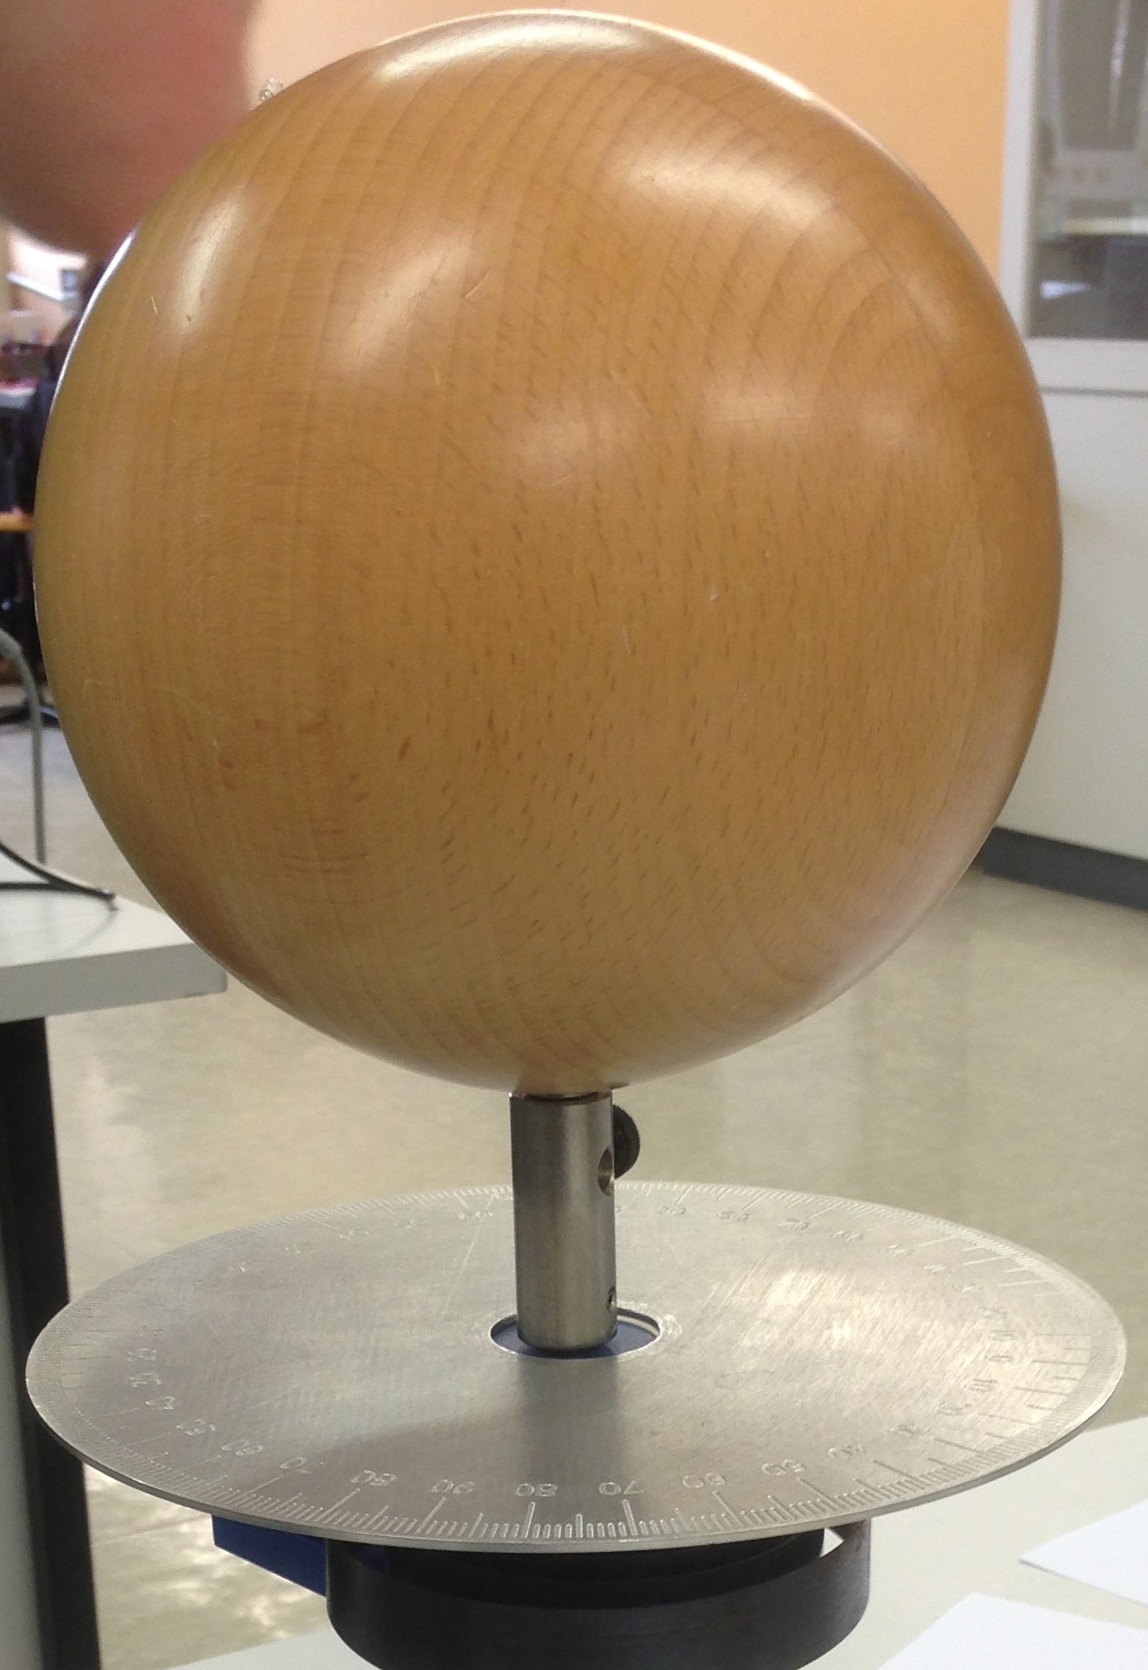
\includegraphics[width = 5cm]{img/kugel.jpg}
						\caption{Kugelk"orper}
						\label{fig:kugel}
					\end{minipage}
				\end{figure}

				\begin{table}[h!]
					\begin{center}
						\caption{Messwerte f"ur die Bestimmung des Tr"agheitsmomentes $I_\mathrm{1, exp}$ der Holzkugel \label{tabelle:kugel}}
						\begin{tabular}{|c||c||c|}
							\hline
							$\overline{T} [\SI{}{\second}]$ & $\overline{T} [\SI{}{\second}]$ & $\overline{T} [\SI{}{\second}]$ \\
							\hline 
							\hline
							1,82 & 1,84 & 1,84 \\
1,82 & 1,87 & 1,82 \\
1,82 & 1,83 & 1,86 \\
1,85 & -    & -    \\











							\hline 
						\end{tabular}
					\end{center}
				\end{table}

				Die Messwerte aus Tabelle \ref{tabelle:kugel} liefern mit Gleichung \eqref{dauer}

				\begin{eqnarray*}
					I_\mathrm{1, exp} & = & \SI{4.96 (2)}{\gram \meter \squared} \,, \\
					\delta_1 & = & \SI{96}{\percent} \,.
				\end{eqnarray*}

			\clearpage
			\subsubsection{Der Messingzylinder}
			\label{subsubsec:holzkugel}
				\begin{figure}[htbp]
					\begin{minipage}[t]{8cm}
						\vspace{0pt}
						Das Tr"agheitsmoment $I_\mathrm{2, t}$ des Zylinders berechnet sich unabh"angig von der H"ohe nach Gleichung \eqref{eqn:zylinder}.

						\begin{eqnarray}
							I_\mathrm{2, t} & = & \frac{1}{2}mr^2 \,, \label{eqn:zylinder} \\
							\Delta I_\mathrm{2, t} & = & \frac{1}{2} \sqrt{ \left(r^2 \Delta m\right)^2 + \left( 2 mr \Delta r\right)^2} \,. \nonumber
						\end{eqnarray}

						Mit den gemessenen Werten f"ur die Masse $m$ und den Radius $r$ folgt

						\begin{eqnarray*}
							m & = & \SI{1436.0 (1)}{\gram} \,, \\
							r & = & \SI{4.25 (5)}{\centi \meter} \,, \\
							\Rightarrow \quad I_\mathrm{2, t} & = & \SI{1.30 (3)}{\gram \meter \squared} \,.
						\end{eqnarray*}

						Tabelle \ref{tabelle:messingzylinder} beinhaltet die Messdaten zur experimentellen Bestimmung:
					\end{minipage}
					\hfill
					\begin{minipage}[t]{5cm}
						\vspace{0pt}
						\centering
						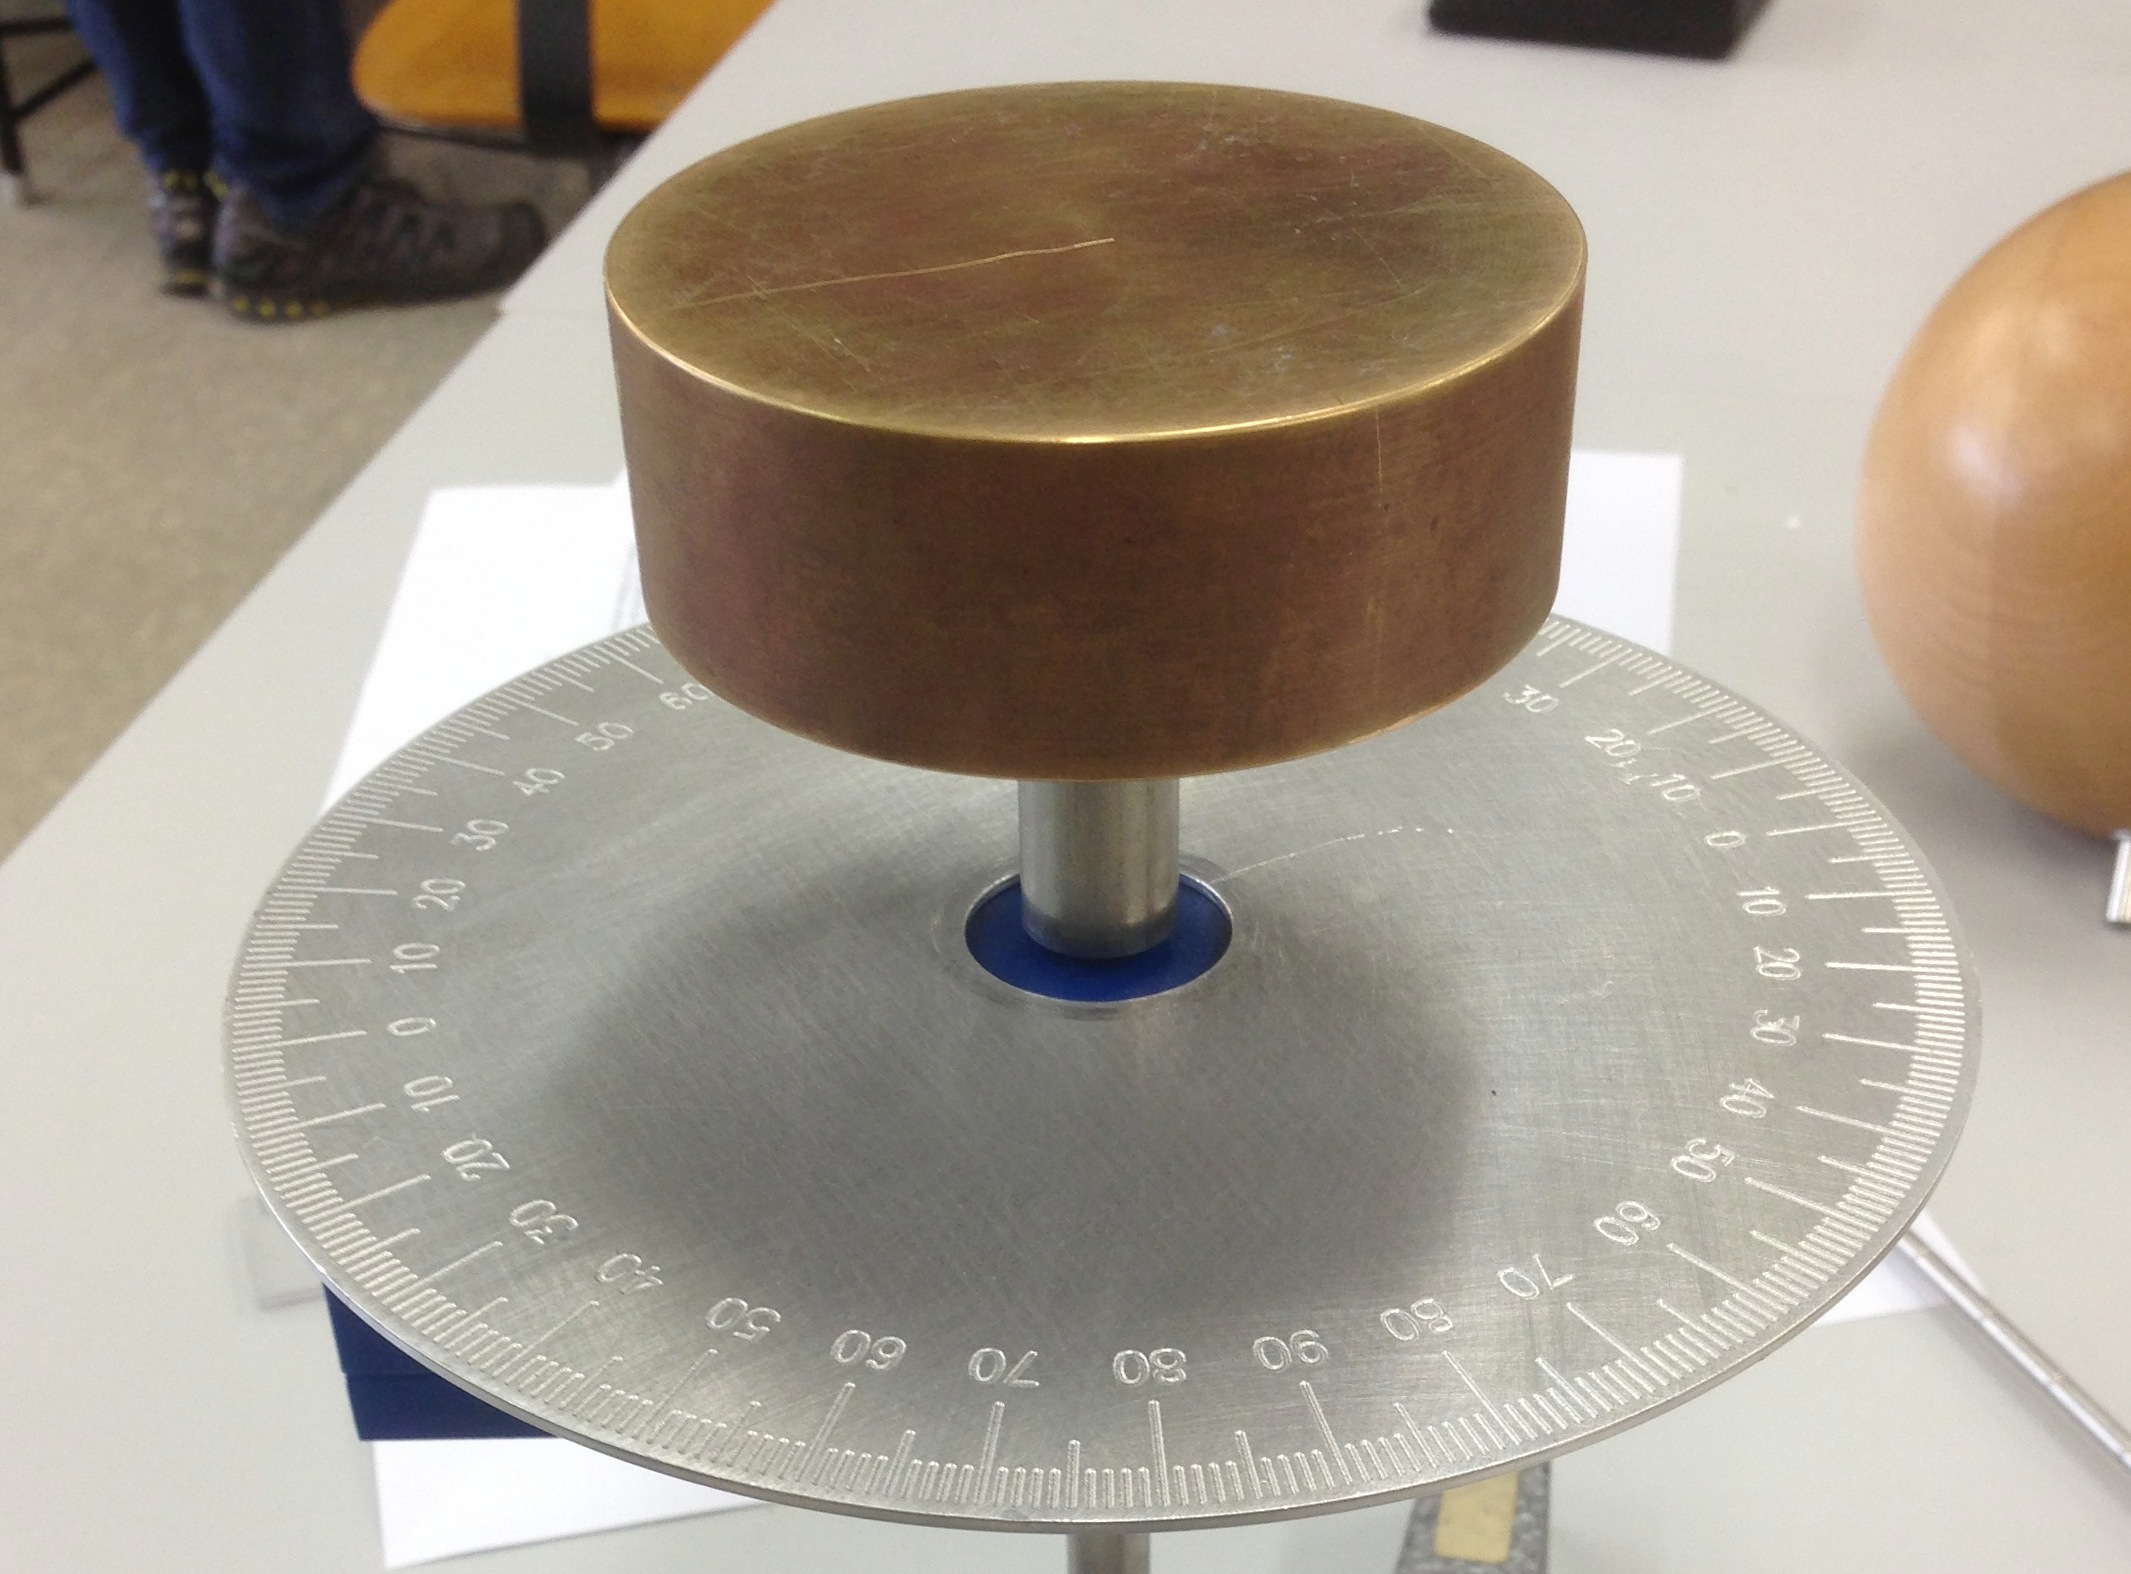
\includegraphics[width = 5cm]{img/messing.jpg}
						\caption{Messingzylinder}
						\label{fig:zylinder}
					\end{minipage}
				\end{figure}

				\begin{table}[h!]
					\begin{center}
						\caption{Messwerte f"ur die Bestimmung des Tr"agheitsmomentes $I_\mathrm{2, exp}$ des Messingzylinders \label{tabelle:messingzylinder}}
						\begin{tabular}{|c||c||c|}
							\hline
							$\overline{T} [\SI{}{\second}]$ & $\overline{T} [\SI{}{\second}]$ & $\overline{T} [\SI{}{\second}]$ \\
							\hline 
							\hline
							1,34 & 1,35 & 1,32 \\
1,35 & 1,34 & 1,32 \\
1,31 & 1,32 & 1,33 \\
1,30 & -    & -    \\











							\hline 
						\end{tabular}
					\end{center}
				\end{table}

				Die Messwerte liefern mit Gleichung \eqref{dauer}

				\begin{eqnarray*}
					I_\mathrm{2, exp} & = & \SI{2.59 (1)}{\gram \meter \squared} \,, \\
					\delta_2 & = & \SI{99}{\percent} \,.
				\end{eqnarray*}

			\clearpage
			\subsubsection{Puppe}
			\label{subsubsec:puppe}
				Die Holzpuppe wird zur Berechnung des Tr"agheitsmomentes n"aherungsweise durch eine Anordnung von Zylindern $Z_\mathrm{i}$ beschrieben.
				Dabei werden Arme, Beine, Torus und Kopf jeweils als Zylinder betrachtet und mit Hilfe des Steinersches Satzes zu einem Gesamttr"agheitsmoment $I$ zusammengesetzt.
				Der Index $i$ ist stets nach den K"orperteilen bennant.

				Kopf und Torus werden durch die Symmetrieachse gedreht.
				Die Beine werden parallel zur Symmetrieachse gedreht und m"ussen daher mit dem Steinerschen Satz verschoben werden.
				Ebenso werden die Arme in der ersten Position der Puppe parallel und in der zweiten Position im rechten Winkel zur Symmetrieachse gedreht. Die Stellungen der Puppe sind in Abbildung \ref{fig:puppe1} und \ref{fig:puppe2} verdeutlicht.

				% Alle Zylinderradien $r_\mathrm{i}$ werden "uber zehn Messwerte an verschiedenen Stellen des jeweiligen K"orperteils gemittelt.
				% F"u"se und H"ande werden mit jeweils einem Messwert zu den Beinen, beziehungsweise Armen gez"ahlt.

				\begin{figure}[h]
					\begin{minipage}[t]{7cm}
						\vspace{0pt}
						\centering
						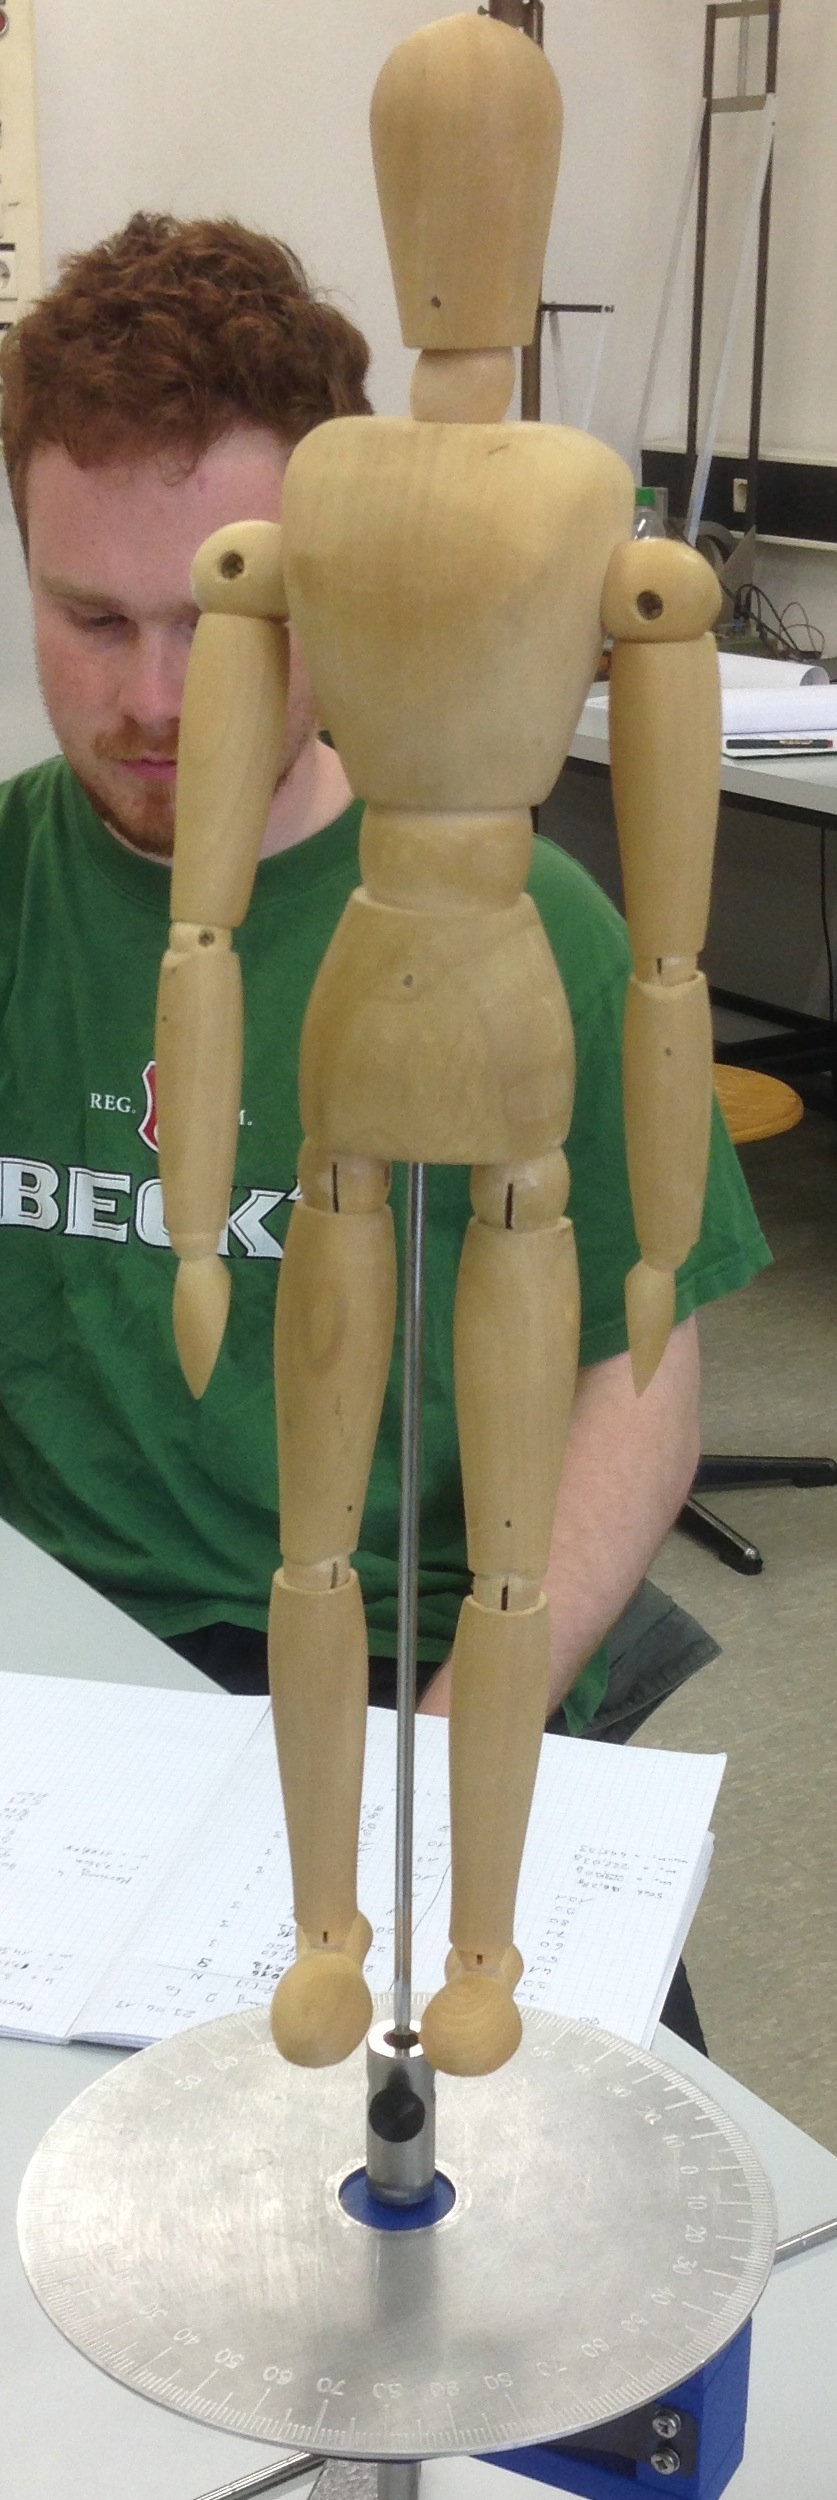
\includegraphics[height = 7cm]{img/pupp1.jpg}
						\caption{Puppe in Stellung 1}
						\label{fig:puppe1}
					\end{minipage}
					\hfill
					\begin{minipage}[t]{7cm}
						\vspace{0pt}
						\centering
						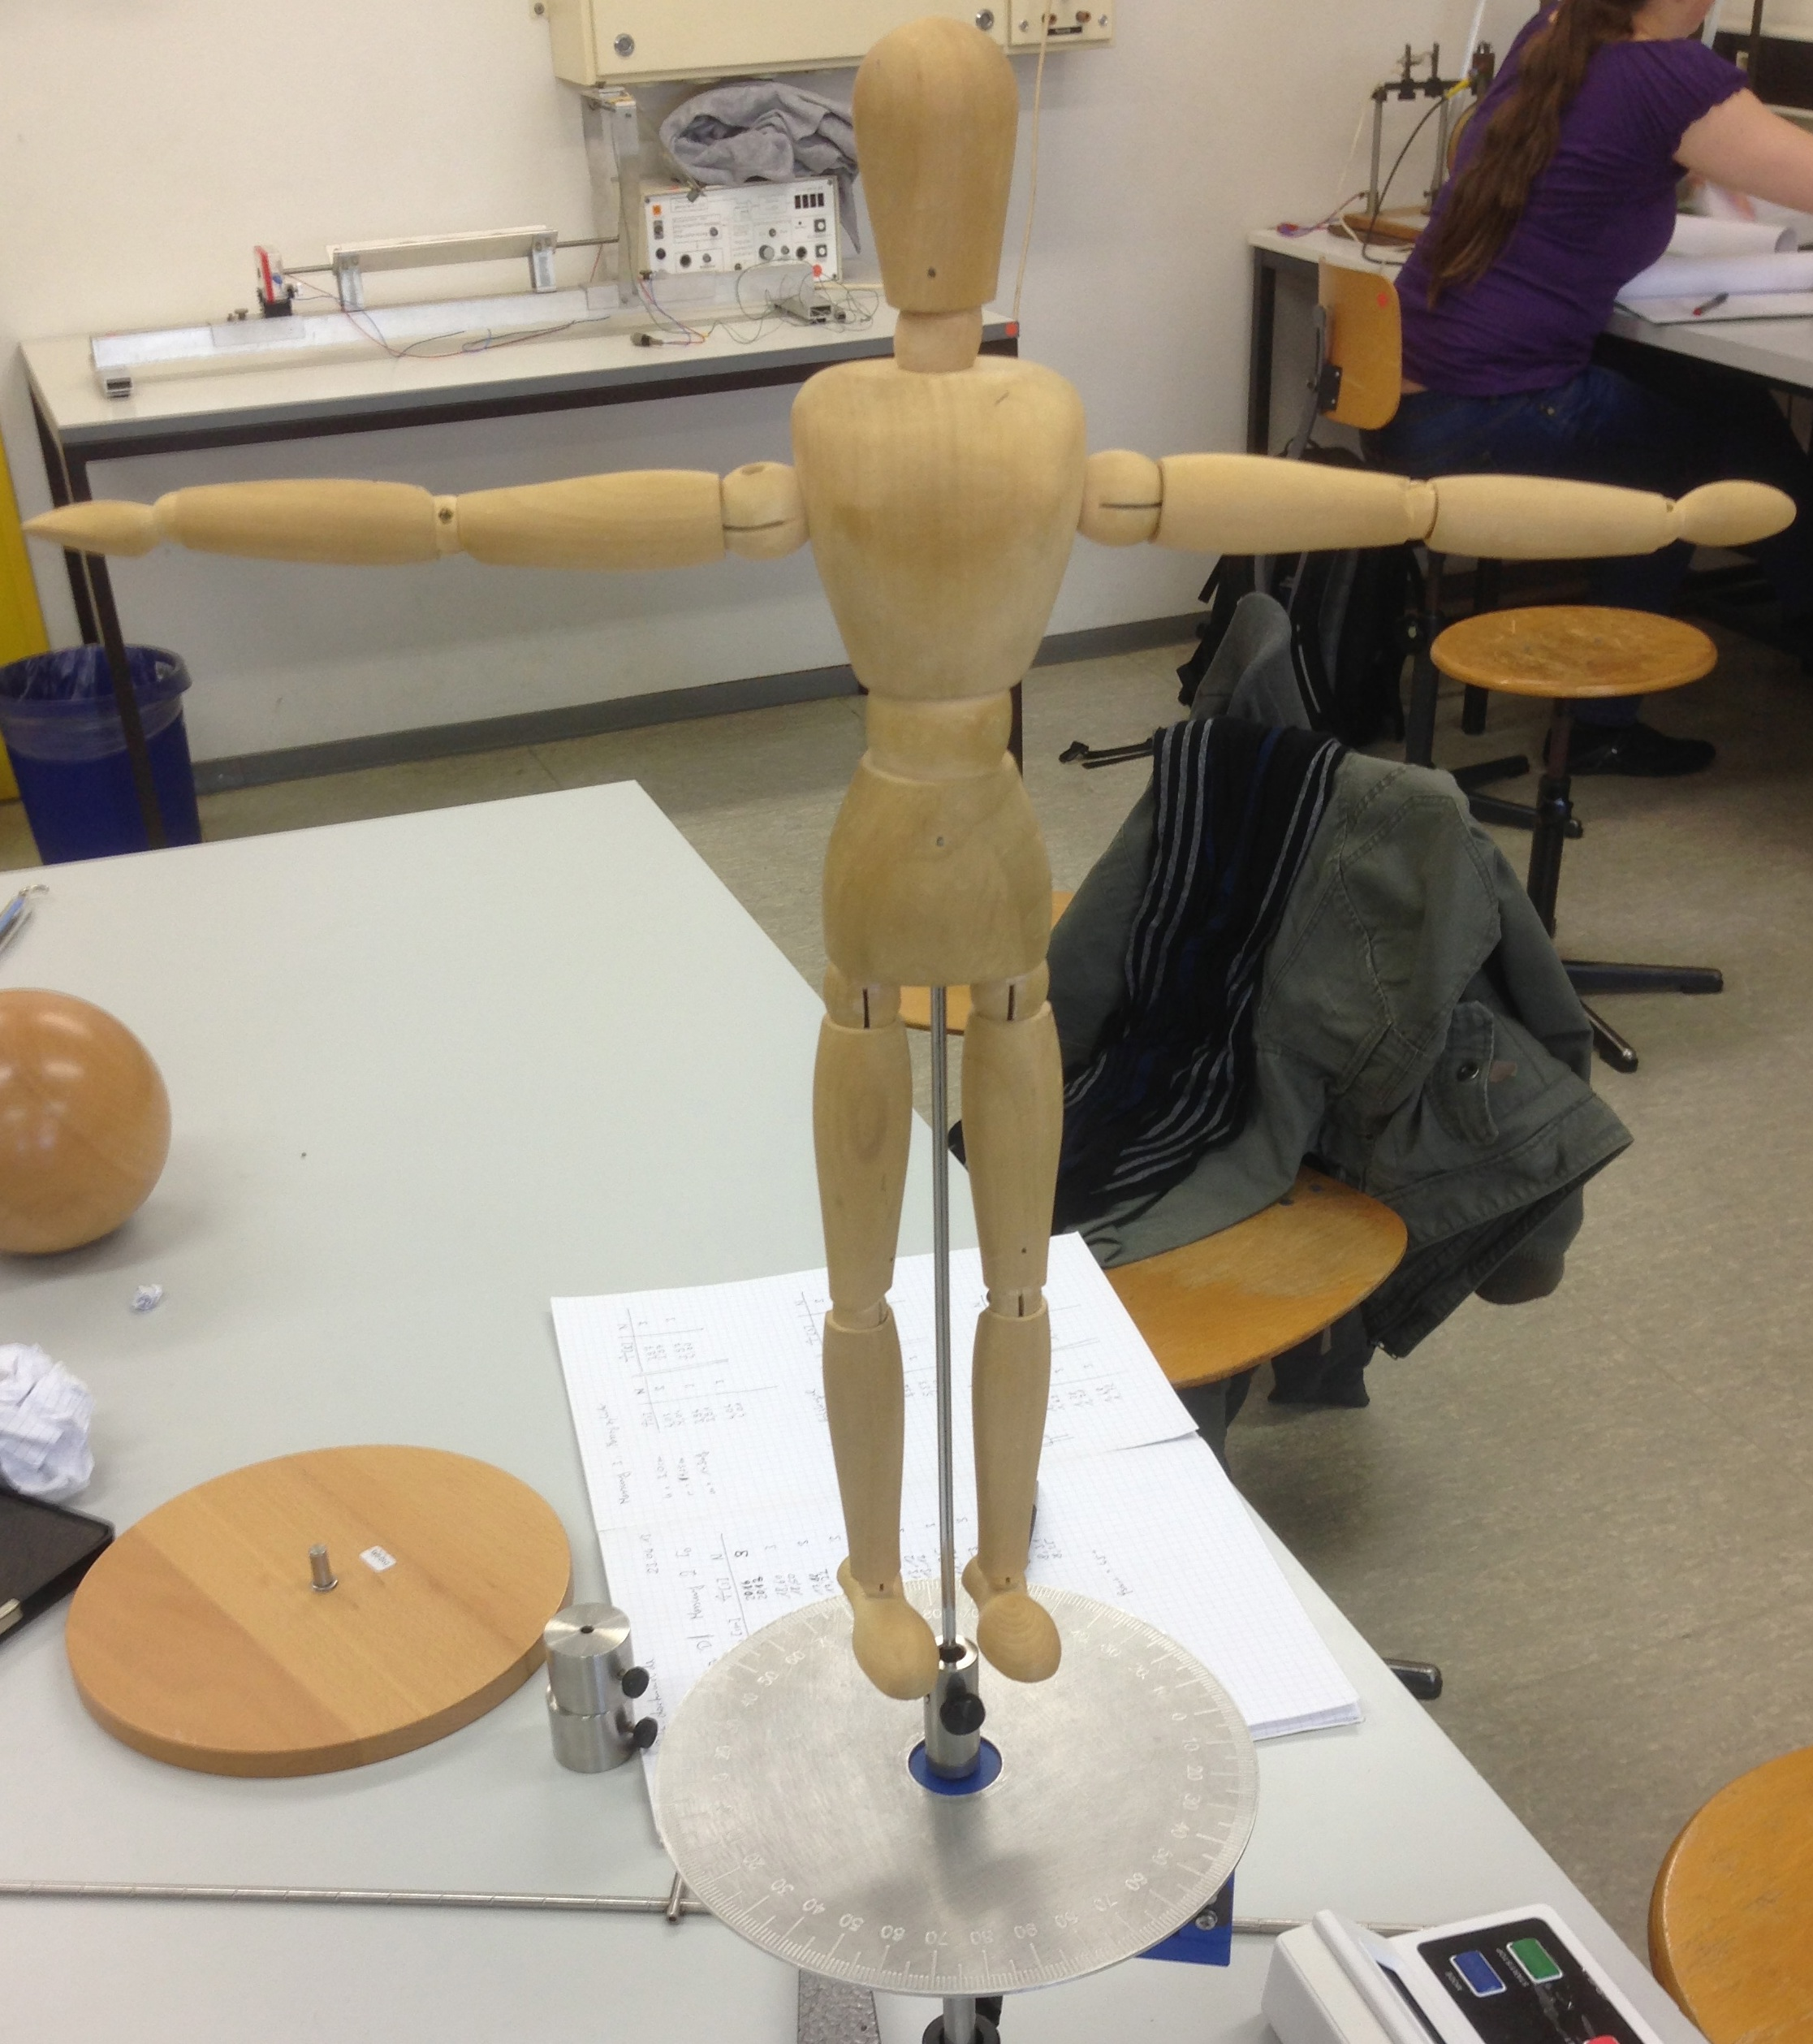
\includegraphics[height = 7cm]{img/pupp2.jpg}
						\caption{Puppe in Stellung 2}
						\label{fig:puppe2}
					\end{minipage}
				\end{figure}

				Die einzelnen Massen $m_\mathrm{i}$ werden dabei aus der Dichte $\rho = M / V = \SI{.743}{\gram \per \centi \meter \cubed}$ mit der Gesamtmasse $M$ und dem Gesamtvolumen $V$ bestimmt:

				\begin{eqnarray*}
					M = \SI{340.75}{\gram} & , & V = \SI{458.8}{\centi \meter \cubed} \\
					\Rightarrow \rho & = & \SI{.743}{\gram \per \centi \meter \cubed}
				\end{eqnarray*}

				F"ur $I$ gilt damit

				\begin{eqnarray*}
					I & = & I_\mathrm{Kopf} + I_\mathrm{Torus} + 2 I_\mathrm{Arm} + 2 I_\mathrm{Bein} + 2 m_\mathrm{Arm}a_\mathrm{Arm}^2 + 2 m_\mathrm{Bein}a_\mathrm{Bein}^2 \,, \\
					\Delta I & = & \left[(\Delta I_\mathrm{K})^2 + (\Delta I_\mathrm{T})^2 + (2 \Delta I_\mathrm{A})^2 + 2(\Delta I_\mathrm{B})^2 +\right. \\
					&& \left. + (2a_\mathrm{A}^2 \Delta m_\mathrm{A})^2 + (4 a_\mathrm{A}m_\mathrm{A} \Delta a_\mathrm{A})^2 + (2a_\mathrm{B}^2 \Delta m_\mathrm{B})^2 + (4 a_\mathrm{B}m_\mathrm{B} \Delta a_\mathrm{B})^2\right]^\frac{1}{2} \,.
				\end{eqnarray*}

				Ausserdem gilt

				\begin{eqnarray*}
					V_\mathrm{i} & = & \pi r_\mathrm{i}^2 h_\mathrm{i} \,, \\
					\Delta V_\mathrm{i} & = & \pi \sqrt{(r_\mathrm{i} h_\mathrm{i} \Delta r_\mathrm{i})^2 + (r_\mathrm{i}^2 \Delta h_\mathrm{i})} \, \\
				\end{eqnarray*}

				und $I_\mathrm{i}$ in Stellung 1 wie in Gleichung \eqref{eqn:zylinder} beschrieben. In Stellung 2 gilt

				\begin{eqnarray*}
					I_\mathrm{Arm} & = & \frac{1}{4}m_\mathrm{Arm}r_\mathrm{Arm}^2 + \frac{1}{12}m_\mathrm{Arm}h_\mathrm{Arm}^2 \,, \\
					\Delta I_\mathrm{Arm} & = & \sqrt{\left(\frac{1}{4}r_\mathrm{A}^2 + \frac{1}{12}h_\mathrm{A}^2\right)^2 \Delta m_\mathrm{A}^2 + \left(\frac{1}{2}m_\mathrm{A}r_\mathrm{A}\Delta r_\mathrm{A}\right)^2 + \left(\frac{1}{6}m_\mathrm{A}h_\mathrm{A}\Delta h_\mathrm{A}\right)^2}
				\end{eqnarray*}

				Mit $a_\mathrm{Arm} = r_\mathrm{Torus} + r_\mathrm{Arm}$ und $a_\mathrm{Bein} = \SI{3.00 (5)}{\centi \meter}$ folgt f"ur Stellung 1

				\begin{equation*}
					I_1 = \SI{1.96 (16)}{\kilo \gram \centi \meter \squared} \,.
				\end{equation*}

				Mit $a_\mathrm{Arm} = r_\mathrm{Torus} + h_\mathrm{Arm} / 2$ folgt f"ur Stellung 2

				\begin{equation*}
					I_2 = \SI{8.91 (17)}{\kilo \gram \centi \meter \squared} \,.
				\end{equation*}

				Die Messdaten aus den Tabellen \ref{tabelle:puppeneigenschaften} und \ref{tabelle:puppe} liefern mit Gleichung \eqref{dauer} die Ergebnisse

				\begin{eqnarray*}
					I_1 & = & \SI{1.84 (15)}{\kilo \gram \centi \meter \squared} \,, \\
					I_2 & = & \SI{5.02 (30)}{\kilo \gram \centi \meter \squared} \,, \\
					\delta_1 & = & \SI{6.1}{\percent} \,, \\
					\delta_2 & = & \SI{43.7}{\percent} \,.
				\end{eqnarray*}

				\clearpage

				\begin{table}[h!]
					\begin{center}
						\caption{Durchmesser der zylinderf"ormigen K"orperteile der Puppe \label{tabelle:puppenradien}}
						\begin{tabular}{|c|c|c|c|}
							\hline
							$d_\mathrm{Kopf} [\SI{}{\milli \meter}]$ & $d_\mathrm{Torus} [\SI{}{\milli \meter}]$ & $d_\mathrm{Arm} [\SI{}{\milli \meter}]$ & $d_\mathrm{Bein} [\SI{}{\milli \meter}]$ \\
							\hline 
							\hline
							$\SI{32.0}{}$ & $\SI{48.0}{}$ & $\SI{21.0}{}$ & $\SI{25.0}{}$ \\
$\SI{29.0}{}$ & $\SI{50.0}{}$ & $\SI{18.0}{}$ & $\SI{26.0}{}$ \\
$\SI{19.0}{}$ & $\SI{48.0}{}$ & $\SI{12.0}{}$ & $\SI{24.0}{}$ \\
$\SI{18.0}{}$ & $\SI{40.0}{}$ & $\SI{17.0}{}$ & $\SI{23.0}{}$ \\
$\SI{32.0}{}$ & $\SI{32.0}{}$ & $\SI{16.0}{}$ & $\SI{20.0}{}$ \\
$\SI{26.0}{}$ & $\SI{33.0}{}$ & $\SI{10.0}{}$ & $\SI{15.0}{}$ \\
$\SI{29.0}{}$ & $\SI{42.0}{}$ & $\SI{20.0}{}$ & $\SI{19.0}{}$ \\
$\SI{32.0}{}$ & $\SI{51.0}{}$ & $\SI{15.0}{}$ & $\SI{21.0}{}$ \\
$\SI{27.0}{}$ & $\SI{56.0}{}$ & $\SI{16.0}{}$ & $\SI{20.0}{}$ \\
$\SI{26.0}{}$ & $\SI{51.0}{}$ & $\SI{19.0}{}$ & $\SI{17.0}{}$ \\
							\hline 
						\end{tabular}
					\end{center}
					
				\end{table}

				\begin{table}[h!]
					\begin{center}
						\caption{Ben"otigte Eigenschaften der K"orperteile\label{tabelle:puppeneigenschaften}}
						\begin{tabular}{|c||c|c|c|c|c|}
							\hline
								 &
								$r [\SI{}{\milli \meter}]$ &
								$h [\SI{}{\milli \meter}]$ &
								$V [\SI{}{\centi \meter \cubed}]$ &
								$m [\SI{}{\gram}]$ &
								$I [\SI{}{\gram \centi \meter \squared}]$ \\
							\hline 
							\hline
								Kopf &
								$\SI{13.5 (25)}{} $ &
								$\SI{65.0 (5)}{}$ &
								$\SI{37.2 (69)}{}$&
								$\SI{27.6 (10)}{}$&
								$\SI{25.2 (93)}{}$\\
							\hline 
								Torus &
								$\SI{22.6 (40)}{} $ &
								$\SI{133.0 (5)}{}$ &
								$\SI{213.4 (378)}{}$&
								$\SI{171.8 (10)}{}$&
								$\SI{438.8 (1553)}{}$\\
							\hline 
								Arm 1 &
								$\SI{8.2 (17)}{}$ &
								$\SI{170.0 (5)}{}$ &
								$\SI{35.9 (74)}{}$&
								$\SI{26.7 (10)}{}$&
								$\SI{9.0 (37)}{}$\\
							\hline 
								Arm 2 &
								$\SI{8.2 (17)}{}$ &
								$\SI{170.0 (5)}{}$ &
								$\SI{35.9 (74)}{}$&
								$\SI{26.7 (10)}{}$&
								$\SI{646.5 (246)}{}$\\
							\hline 
								Bein &
								$\SI{10.5 (18)}{}  $& 
								$\SI{197.0 (5)}{}$ &
								$\SI{68.2 (117)}{}$&
								$\SI{50.7 (10)}{}$&
								$\SI{27.9 (96)}{}$\\
							\hline
							\hline
								 &
								\multicolumn{5}{c|}{$I_1 = \SI{1.96 (16)}{\kilo \gram \centi \meter \squared}$ \quad , \quad $I_2 = \SI{8.91 (17)}{\kilo \gram \centi \meter \squared}$} \\
							\hline
						\end{tabular}
					\end{center}
				\end{table}

				\begin{table}[h!]
					\begin{center}
						\caption{Schwingungsdauern der Puppe\label{tabelle:puppe}}
						\begin{tabular}{|c||c||c||c|}
							\hline
							$\overline{T_1} [\SI{}{\second}]$ & $\overline{T_1} [\SI{}{\second}]$ & $\overline{T_2} [\SI{}{\second}]$ & $\overline{T_2} [\SI{}{\second}]$ \\
							\hline 
							\hline
							0,57 & 0,57 & 0,96 & 0,96 \\
0,56 & 0,54 & 0,96 & 0,89 \\
0,59 & 0,53 & 0,98 & 0,96 \\
0,57 & 0,60 & 0,97 & 0,94 \\
0,56 & 0,61 & 0,89 & 0,94 \\
							\hline 
						\end{tabular}
					\end{center}
				\end{table}

				\clearpage
